\documentclass[aspectratio=169]{beamer}

% =================================================================
%  Structures and Data Structures in C
%  A beginner-friendly Beamer deck (fully self-contained: all
%  figures / diagrams drawn with TikZ, so it compiles anywhere).
%  Style mirrors "c-programming-intro.tex".
% =================================================================

% -------------------------------------------------
% Theme and packages
% -------------------------------------------------
\usetheme{Madrid}
\usecolortheme{default}

\usepackage{amsmath}
\usepackage{amssymb}
\usepackage{bm}
\usepackage{listings}
\usepackage{tikz}
\usepackage{array}
\usepackage{booktabs}
\usepackage{tabularx}
\usepackage{ragged2e}
\usepackage{xcolor}

\usetikzlibrary{shapes.geometric, arrows.meta, positioning, calc, fit, backgrounds, trees}

% -------------------------------------------------
% Colour palette
% -------------------------------------------------
\definecolor{cAccent}{RGB}{0,102,153}     % teal-blue accent
\definecolor{cBox}{RGB}{28,31,42}          % dark box
\definecolor{cGreen}{RGB}{34,139,34}
\definecolor{cRed}{RGB}{178,34,34}
\definecolor{cOrange}{RGB}{204,102,0}
\definecolor{cPurple}{RGB}{102,45,145}
\definecolor{cGrayBg}{RGB}{245,246,248}
\definecolor{codebg}{RGB}{248,248,244}
\definecolor{codekw}{RGB}{0,0,180}
\definecolor{codecomment}{RGB}{0,130,0}
\definecolor{codestr}{RGB}{170,55,20}

% Beamer colour tweaks (match a Madrid-style accent)
\setbeamercolor{structure}{fg=cAccent}
\setbeamertemplate{frametitle continuation}{%
	\ifnum\insertcontinuationcount>1\space(cont...)\fi
}
\setbeamertemplate{navigation symbols}{}
\setbeamertemplate{caption}[numbered]

% -------------------------------------------------
% Listings style for C code
% -------------------------------------------------
\lstdefinestyle{cstyle}{
	language=C,
	backgroundcolor=\color{codebg},
	basicstyle=\ttfamily\footnotesize,
	keywordstyle=\color{codekw}\bfseries,
	commentstyle=\color{codecomment}\itshape,
	stringstyle=\color{codestr},
	numbers=none,
	numberstyle=\tiny\color{gray},
	numbersep=8pt,
	showstringspaces=false,
	breaklines=true,
	frame=single,
	rulecolor=\color{gray!50},
	tabsize=2,
	columns=fullflexible,
	keepspaces=true,
	literate={~}{{$\sim$}}1
}
\lstset{style=cstyle}

% Handy TikZ node styles
\tikzset{
	startstop/.style={rectangle, rounded corners=10pt, minimum width=2.4cm, minimum height=0.8cm, text centered, align=center, draw=black, fill=cAccent!25},
	process/.style  ={rectangle, minimum width=2.6cm, minimum height=0.8cm, text centered, align=center, text width=2.8cm, draw=black, fill=blue!8},
	io/.style       ={trapezium, trapezium left angle=70, trapezium right angle=110, minimum width=2.2cm, minimum height=0.8cm, text centered, align=center, draw=black, fill=cOrange!20},
	decision/.style ={diamond, aspect=2, minimum width=2.4cm, minimum height=0.9cm, text centered, text width=2.2cm, draw=black, fill=cGreen!18, inner sep=1pt},
	flowarrow/.style={-{Stealth[length=2.5mm]}, thick},
	% memory-cell helpers
	acell/.style={draw=black, minimum width=1.05cm, minimum height=1.0cm, text centered, font=\small, fill=blue!8},
	scell/.style={draw=black, minimum width=1.7cm, minimum height=0.75cm, text centered, font=\small, fill=blue!8},
	treenode/.style={circle, draw, minimum size=0.72cm, inner sep=1pt, font=\small, fill=cAccent!15},
}

\setbeamertemplate{footnote}{%
	\parindent 0em
	\noindent
	\raggedright
	\insertfootnotemark\insertfootnotetext\par
}

% -------------------------------------------------
% Title information
% -------------------------------------------------
\title[Structures \& Data Structures]{Structures and Data Structures in C}
\subtitle{Records, Unions, Stacks, Queues, and Trees}
\author[Amit Kumar Singh]{}
\institute[]{
	Amit Kumar Singh \\
	\vspace{0.1cm}
	Assistant Professor (ECE) \\
	\vspace{0.05cm}
	School of Naval Architecture and Ocean Engineering\\
	\vspace{0.05cm}
	Indian Maritime University Visakhapatnam Campus, Sabbavaram Mandal\\
	\vspace{0.05cm}
	Visakhapatnam, Andhra Pradesh -- 531~035\\
	\vspace{0.25cm}
	amitkumarsingh@imu.ac.in
}
\date[Programming in C]{\today}

\begin{document}

	%------------------------------------------------
	\begin{frame}
		\titlepage
	\end{frame}

	%------------------------------------------------
	\begin{frame}{Outline}
		\small
		\begin{columns}[T,onlytextwidth]
			\hspace{0.8cm}
			\begin{column}{0.49\textwidth}
				\tableofcontents[hideallsubsections, sections={1-5}]
			\end{column}
			\hspace{0.8cm}
			\begin{column}{0.42\textwidth}
				\tableofcontents[hideallsubsections, sections={6-9}]
			\end{column}
		\end{columns}
	\end{frame}

	% =================================================================
	\section{Introduction to Structures}
	% =================================================================
	\begin{frame}{Why Do We Need Structures?}
		\begin{block}{The problem}
			An array stores many items of the \textbf{same} type. But a real record --- say a
			\textbf{student} --- mixes a name (\texttt{char[]}), a roll number (\texttt{int}) and marks
			(\texttt{float}). Separate variables for each field quickly become unmanageable.
		\end{block}
		\begin{columns}[T]
			\begin{column}{0.5\textwidth}
				\begin{block}{Without structures}
					\small Three loose variables per student: \texttt{name1}, \texttt{roll1}, \texttt{marks1}, \dots
					--- no link between them.
				\end{block}
			\end{column}
			\begin{column}{0.5\textwidth}
				\begin{block}{With a structure}
					\small One named record \texttt{Student} bundles all fields together, so they travel as a
					single unit.
				\end{block}
			\end{column}
		\end{columns}
		\vspace{0.15cm}
		\centering\footnotesize A \textbf{structure} groups related values of \emph{different} types under one name.
	\end{frame}

	\begin{frame}{What is a Structure?}
		\begin{block}{Definition}
			A \textbf{structure} is a user-defined data type that groups \textbf{several variables}
			(possibly of different types), called \textbf{members} or \textbf{fields}, under a single name.
		\end{block}
		\vspace{0.1cm}
		\centering
		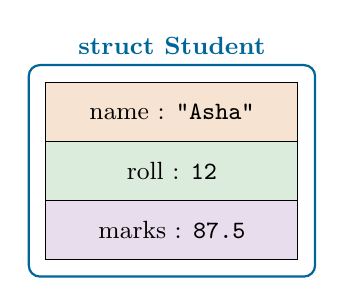
\begin{tikzpicture}[font=\small]
			\node[scell, fill=cOrange!18, minimum width=3.2cm] (n) at (0,1.5) {name : \texttt{"Asha"}};
			\node[scell, fill=cGreen!16, minimum width=3.2cm]  (r) at (0,0.75) {roll : \texttt{12}};
			\node[scell, fill=cPurple!16, minimum width=3.2cm] (m) at (0,0.0) {marks : \texttt{87.5}};
			\begin{scope}[on background layer]
				\node[draw=cAccent, thick, rounded corners, fit=(n)(r)(m), inner sep=6pt,
				label={[cAccent]above:\textbf{struct Student}}] {};
			\end{scope}
		\end{tikzpicture}
		\vspace{0.1cm}
		\begin{itemize}\small
			\item Each member has its own name and type.
			\item The whole record is treated as one object you can copy, pass, and store.
		\end{itemize}
	\end{frame}

	% =================================================================
	\section{Declaration, Definition \& Initialization}
	% =================================================================
	\begin{frame}[fragile]{Declaring and Defining Structures}
		\begin{columns}[T]
			\begin{column}{0.52\textwidth}
				\begin{lstlisting}
/* 1. define the template (a new type) */
struct Student {
    char  name[20];
    int   roll;
    float marks;
};        /* note the semicolon */

/* 2. create variables of that type */
struct Student s1, s2;
				\end{lstlisting}
			\end{column}
			\begin{column}{0.48\textwidth}
				\begin{block}{Cleaner names with \texttt{typedef}}
					\small
				\end{block}
				\begin{lstlisting}
typedef struct {
    int day, month, year;
} Date;

Date today;   /* no "struct" needed */
				\end{lstlisting}
				\footnotesize The template itself uses \textbf{no memory}; each \emph{variable} does.
			\end{column}
		\end{columns}
	\end{frame}

	\begin{frame}[fragile]{Initializing Structures}
		\begin{columns}[T]
			\begin{column}{0.55\textwidth}
				\begin{lstlisting}
/* positional order */
struct Student s1 = {"Asha", 12, 87.5};

/* designated initializers (any order) */
struct Student s2 = {.roll = 5,
                     .name = "Ravi",
                     .marks = 76.0};

/* member-by-member */
struct Student s3;
strcpy(s3.name, "Meera");
s3.roll  = 9;
s3.marks = 91.0;
				\end{lstlisting}
			\end{column}
			\begin{column}{0.45\textwidth}
				\begin{itemize}\small
					\item \textbf{Positional} values fill the members in order.
					\item \textbf{Designated} initializers name each field --- clear and order-free.
					\item Strings are copied with \texttt{strcpy}, not \texttt{=}.
				\end{itemize}
			\end{column}
		\end{columns}
	\end{frame}

	% =================================================================
	\section{Accessing Structures}
	% =================================================================
	\begin{frame}[fragile]{Accessing Members: \texttt{.} and \texttt{->}}
		\begin{columns}[T]
			\begin{column}{0.55\textwidth}
				\begin{lstlisting}
struct Student s1 = {"Asha", 12, 87.5};

/* dot operator on a variable */
printf("%s\n", s1.name);
s1.roll = 15;

/* arrow operator through a pointer */
struct Student *p = &s1;
printf("%d\n", p->roll);   /* 15 */
p->marks = 90.0;           /* same as (*p).marks */
				\end{lstlisting}
			\end{column}
			\begin{column}{0.45\textwidth}
				\renewcommand{\arraystretch}{1.3}
				\centering
				\begin{tabular}{@{}cl@{}}
					\toprule
					\textbf{Operator} & \textbf{Use with} \\
					\midrule
					\texttt{.}  & a structure \emph{variable} \\
					\texttt{->} & a \emph{pointer} to structure \\
					\bottomrule
				\end{tabular}
				\vspace{0.2cm}
				\begin{block}{Shortcut}
					\small \texttt{p->roll} is just easier-to-read \texttt{(*p).roll}.
				\end{block}
			\end{column}
		\end{columns}
	\end{frame}

	% =================================================================
	\section{Structures and Functions}
	% =================================================================
	\begin{frame}[fragile]{Passing Structures to Functions}
		\begin{columns}[T]
			\begin{column}{0.55\textwidth}
				\begin{lstlisting}
struct Point { int x, y; };

/* by value: works on a COPY */
void show(struct Point p) {
    printf("(%d, %d)\n", p.x, p.y);
}

/* by pointer: edits the ORIGINAL */
void moveRight(struct Point *p) {
    p->x += 1;
}
				\end{lstlisting}
			\end{column}
			\begin{column}{0.45\textwidth}
				\centering
				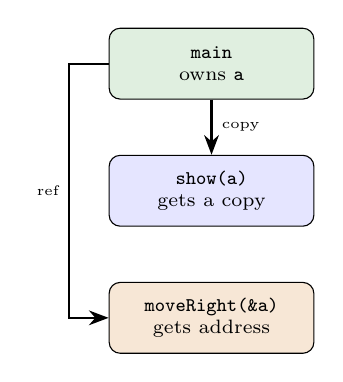
\begin{tikzpicture}[font=\scriptsize,
					b/.style={draw, rounded corners, align=center, minimum height=0.9cm, minimum width=2.6cm}]
					\node[b, fill=cGreen!14] (m) {\texttt{main}\\ owns \texttt{a}};
					\node[b, fill=blue!10, below=0.7cm of m] (v) {\texttt{show(a)}\\ gets a copy};
					\node[b, fill=cOrange!16, below=0.7cm of v] (r) {\texttt{moveRight(\&a)}\\ gets address};
					\draw[flowarrow] (m) -- node[right,font=\tiny]{copy} (v);
					\draw[flowarrow] (m.west) -- ++(-0.5,0) |- node[left,font=\tiny,pos=0.25]{ref} (r.west);
				\end{tikzpicture}
			\end{column}
		\end{columns}
		\vspace{0.1cm}
		\centering\footnotesize Pass \textbf{by pointer} for big structures (no copy) or when the function must \emph{change} them.
	\end{frame}

	\begin{frame}[fragile]{Structures in Functions: A Full Example}
		\begin{columns}[T]
			\begin{column}{0.58\textwidth}
				\begin{lstlisting}
#include <stdio.h>

struct Point { int x, y; };

void show(struct Point p) {
    printf("(%d, %d)\n", p.x, p.y);
}
void moveRight(struct Point *p) { p->x += 1; }

int main(void)
{
    struct Point a = {3, 4};
    show(a);            /* (3, 4) */
    moveRight(&a);
    show(a);            /* (4, 4) */
    return 0;
}
				\end{lstlisting}
			\end{column}
			\begin{column}{0.42\textwidth}
				\begin{block}{Trace}
					\small
					\begin{itemize}
						\item \texttt{a = (3,4)}.
						\item \texttt{show(a)} prints a copy.
						\item \texttt{moveRight(\&a)} edits \texttt{a.x}.
						\item \texttt{a = (4,4)}.
					\end{itemize}
				\end{block}
				\centering\footnotesize Output:\; \fbox{\parbox{2.4cm}{\ttfamily (3, 4)\\ (4, 4)}}
			\end{column}
		\end{columns}
	\end{frame}

	% =================================================================
	\section{Self-Referential Structures \& Unions}
	% =================================================================
	\begin{frame}[fragile]{Self-Referential Structures}
		\begin{block}{Definition}
			A \textbf{self-referential structure} contains a \textbf{pointer to its own type}. This is
			the building block of \textbf{linked lists}, stacks, queues, and trees.
		\end{block}
		\begin{columns}[T]
			\begin{column}{0.46\textwidth}
				\begin{lstlisting}
struct Node {
    int data;
    struct Node *next; /* same type! */
};
				\end{lstlisting}
			\end{column}
			\begin{column}{0.54\textwidth}
				\centering
				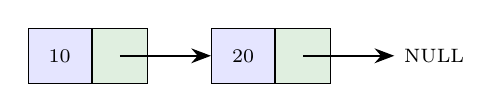
\begin{tikzpicture}[font=\scriptsize, node distance=0.4cm,
					nd/.style={draw, minimum height=0.7cm}]
					\node[nd, minimum width=0.8cm, fill=blue!10] (d1) {10};
					\node[nd, minimum width=0.7cm, right=0cm of d1, fill=cGreen!14] (p1) {\;};
					\node[nd, minimum width=0.8cm, right=0.8cm of p1, fill=blue!10] (d2) {20};
					\node[nd, minimum width=0.7cm, right=0cm of d2, fill=cGreen!14] (p2) {\;};
					\node[right=0.8cm of p2] (nul) {NULL};
					\draw[flowarrow] (p1.center) -- (d2.west);
					\draw[flowarrow] (p2.center) -- (nul.west);
				\end{tikzpicture}
				\vspace{0.15cm}
				\footnotesize Each node holds \textbf{data} and a link (\texttt{next}) to the following node.
			\end{column}
		\end{columns}
	\end{frame}

	\begin{frame}[fragile]{Unions: Sharing One Memory Space}
		\begin{columns}[T]
			\begin{column}{0.5\textwidth}
				\begin{lstlisting}
union Value {
    int   i;
    float f;
    char  c;
};   /* all members share memory */

union Value v;
v.i = 65;
printf("%d\n", v.i);   /* valid */
/* writing v.f now overwrites v.i */
				\end{lstlisting}
				\centering
				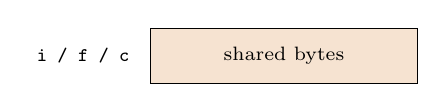
\begin{tikzpicture}[font=\scriptsize]
					\draw[fill=cOrange!18] (0,0) rectangle (3.4,0.7);
					\node at (1.7,0.35) {shared bytes};
					\node at (-0.85,0.35) {\texttt{i / f / c}};
				\end{tikzpicture}
			\end{column}
			\begin{column}{0.5\textwidth}
				\renewcommand{\arraystretch}{1.3}
				\centering
				\begin{tabular}{@{}p{2.2cm}p{2.2cm}@{}}
					\toprule
					\textbf{struct} & \textbf{union} \\
					\midrule
					members have \emph{separate} memory & members \emph{share} memory \\
					size = sum of members & size = largest member \\
					all usable at once & one member at a time \\
					\bottomrule
				\end{tabular}
				\vspace{0.15cm}
				\footnotesize Unions save space when only \emph{one} of several fields is needed at a time.
			\end{column}
		\end{columns}
	\end{frame}

	% =================================================================
	\section{Introduction to Data Structures}
	% =================================================================
	\begin{frame}{What are Data Structures?}
		\begin{block}{Definition}
			A \textbf{data structure} is a systematic way of \textbf{organizing and storing data} so that
			it can be used \textbf{efficiently} --- searched, inserted, deleted, and traversed.
		\end{block}
		\centering
		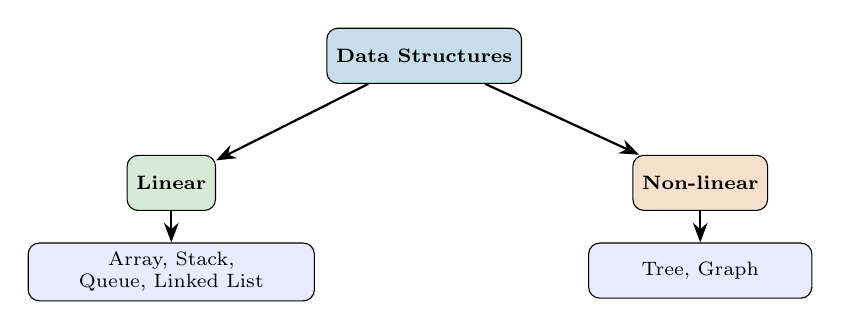
\begin{tikzpicture}[font=\scriptsize,
			b/.style={draw, rounded corners, fill=blue!8, minimum height=0.7cm, align=center},
			hd/.style={draw, rounded corners, fill=cAccent!22, minimum height=0.7cm, align=center, font=\bfseries\scriptsize}]
			\node[hd] (ds) {Data Structures};
			\node[hd, below left=0.9cm and 1.4cm of ds, fill=cGreen!18] (lin) {Linear};
			\node[hd, below right=0.9cm and 1.4cm of ds, fill=cOrange!20] (non) {Non-linear};
			\draw[flowarrow] (ds) -- (lin);
			\draw[flowarrow] (ds) -- (non);
			\node[b, below=0.4cm of lin, text width=3.4cm] (linc) {Array, Stack, Queue, Linked List};
			\node[b, below=0.4cm of non, text width=2.6cm] (nonc) {Tree, Graph};
			\draw[flowarrow] (lin) -- (linc);
			\draw[flowarrow] (non) -- (nonc);
		\end{tikzpicture}
		\vspace{0.1cm}
		\begin{itemize}\small
			\item \textbf{Linear} --- elements in a sequence (one after another).
			\item \textbf{Non-linear} --- elements form a hierarchy or network.
		\end{itemize}
	\end{frame}

	\begin{frame}{Common Operations \& Why They Matter}
		\begin{columns}[T]
			\begin{column}{0.52\textwidth}
				\begin{block}{Typical operations}
					\begin{itemize}\small
						\item \textbf{Traversal} --- visit every element.
						\item \textbf{Insertion} --- add a new element.
						\item \textbf{Deletion} --- remove an element.
						\item \textbf{Searching} --- find an element.
						\item \textbf{Sorting} --- arrange elements in order.
					\end{itemize}
				\end{block}
			\end{column}
			\begin{column}{0.48\textwidth}
				\begin{block}{Why choose carefully}
					\small The right data structure makes these operations \textbf{fast} and the program
					\textbf{simple}. The wrong one makes them slow and clumsy.
				\end{block}
				\centering\footnotesize We now build three classics using \textbf{arrays}: \emph{stack}, \emph{queue}, \emph{tree}.
			\end{column}
		\end{columns}
	\end{frame}

	% =================================================================
	\section{Stacks}
	% =================================================================
	\begin{frame}{Stacks: Last In, First Out (LIFO)}
		\begin{block}{Concept}
			A \textbf{stack} allows adding and removing only at \textbf{one end}, the \textbf{top} ---
			like a pile of plates. The \textbf{last} item pushed is the \textbf{first} popped.
		\end{block}
		\begin{columns}[T]
			\begin{column}{0.45\textwidth}
				\centering\vspace{0.1cm}
				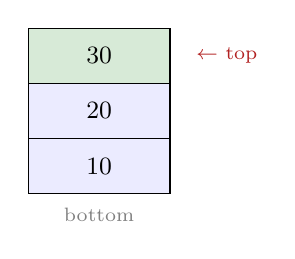
\begin{tikzpicture}[cell/.style={draw, minimum width=1.8cm, minimum height=0.7cm, fill=blue!8, font=\small}]
					\node[cell] (a) at (0,0)   {10};
					\node[cell] (b) at (0,0.7) {20};
					\node[cell, fill=cGreen!18] (c) at (0,1.4) {30};
					\node[right=0.2cm of c, font=\scriptsize, text=cRed] {$\leftarrow$ top};
					\node[below=0.05cm of a, font=\scriptsize, text=gray] {bottom};
				\end{tikzpicture}
			\end{column}
			\begin{column}{0.55\textwidth}
				\begin{itemize}\small
					\item \textbf{push} --- add an item on top.
					\item \textbf{pop} --- remove the top item.
					\item A variable \texttt{top} marks the current top index.
				\end{itemize}
				\begin{block}{Uses}
					\small Undo features, function-call stack, expression evaluation, backtracking.
				\end{block}
			\end{column}
		\end{columns}
	\end{frame}

	\begin{frame}[fragile]{Stack Using an Array: \texttt{push} and \texttt{pop}}
		\begin{columns}[T]
			\begin{column}{0.58\textwidth}
				\begin{lstlisting}
#define MAX 100
int stack[MAX];
int top = -1;           /* empty stack */

void push(int x) {
    if (top == MAX - 1) { printf("Overflow\n"); return; }
    stack[++top] = x;   /* move up, then store */
}

int pop(void) {
    if (top == -1) { printf("Underflow\n"); return -1; }
    return stack[top--];/* read, then move down */
}
				\end{lstlisting}
			\end{column}
			\begin{column}{0.42\textwidth}
				\begin{itemize}\small
					\item \texttt{top = -1} means the stack is \textbf{empty}.
					\item \textbf{Overflow}: pushing to a full array.
					\item \textbf{Underflow}: popping an empty stack.
					\item Both \texttt{push}/\texttt{pop} are \textbf{O(1)} --- constant time.
				\end{itemize}
			\end{column}
		\end{columns}
	\end{frame}

	% =================================================================
	\section{Queues}
	% =================================================================
	\begin{frame}{Queues: First In, First Out (FIFO)}
		\begin{block}{Concept}
			A \textbf{queue} adds at the \textbf{rear} and removes from the \textbf{front} --- like a line
			at a ticket counter. The \textbf{first} item in is the \textbf{first} out.
		\end{block}
		\centering
		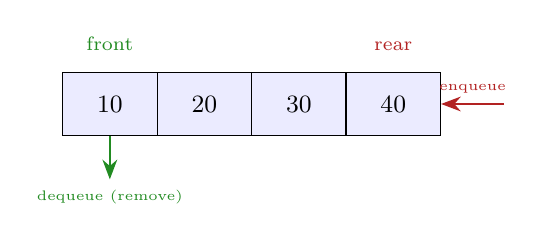
\begin{tikzpicture}[cell/.style={draw, minimum width=1.2cm, minimum height=0.8cm, fill=blue!8, font=\small}]
			\foreach \val/\idx in {10/0, 20/1, 30/2, 40/3} {
				\node[cell] (c\idx) at (\idx*1.2,0) {\val};
			}
			\node[above=0.15cm of c0, font=\scriptsize, text=cGreen] {front};
			\node[above=0.15cm of c3, font=\scriptsize, text=cRed] {rear};
			\draw[flowarrow, cGreen] (c0.south) -- ++(0,-0.55) node[below,font=\tiny]{dequeue (remove)};
			\draw[flowarrow, cRed] ($(c3.east)+(0.8,0)$) -- (c3.east) node[midway,above,font=\tiny]{enqueue};
		\end{tikzpicture}
		\vspace{0.1cm}
		\begin{itemize}\small
			\item \textbf{enqueue} --- add at the rear. \quad \textbf{dequeue} --- remove from the front.
			\item Used in scheduling, buffering, breadth-first search, printer queues.
		\end{itemize}
	\end{frame}

	\begin{frame}[fragile]{Queue Using an Array: \texttt{enqueue} and \texttt{dequeue}}
		\begin{columns}[T]
			\begin{column}{0.58\textwidth}
				\begin{lstlisting}
#define MAX 100
int queue[MAX];
int front = 0, rear = -1;

void enqueue(int x) {
    if (rear == MAX - 1) { printf("Full\n"); return; }
    queue[++rear] = x;      /* add at rear */
}

int dequeue(void) {
    if (front > rear) { printf("Empty\n"); return -1; }
    return queue[front++];  /* remove from front */
}
				\end{lstlisting}
			\end{column}
			\begin{column}{0.42\textwidth}
				\begin{itemize}\small
					\item \texttt{rear} grows on insertion; \texttt{front} grows on removal.
					\item \texttt{front > rear} signals an \textbf{empty} queue.
				\end{itemize}
				\begin{block}{Tip}
					\small A \textbf{circular queue} reuses freed front slots so the array does not ``fill up'' prematurely.
				\end{block}
			\end{column}
		\end{columns}
	\end{frame}

	% =================================================================
	\section{Trees}
	% =================================================================
	\begin{frame}{Trees: A Non-Linear Hierarchy}
		\begin{block}{Concept}
			A \textbf{tree} organizes data in a \textbf{hierarchy} of nodes. Each node may have
			\textbf{children}; the top node is the \textbf{root}. A \textbf{binary tree} allows at most two children.
		\end{block}
		\begin{columns}[T]
			\begin{column}{0.5\textwidth}
				\centering
				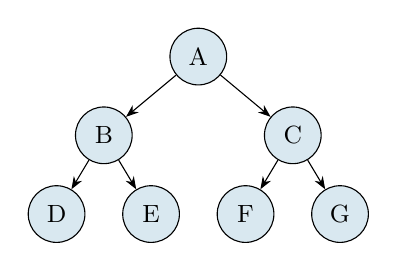
\begin{tikzpicture}[
					level 1/.style={sibling distance=2.4cm},
					level 2/.style={sibling distance=1.2cm},
					edge from parent/.style={draw, -{Stealth[length=1.6mm]}},
					level distance=1cm]
					\node[treenode] {A}
						child {node[treenode] {B} child {node[treenode] {D}} child {node[treenode] {E}}}
						child {node[treenode] {C} child {node[treenode] {F}} child {node[treenode] {G}}};
				\end{tikzpicture}
			\end{column}
			\begin{column}{0.5\textwidth}
				\begin{itemize}\small
					\item \textbf{Root} --- topmost node (\texttt{A}).
					\item \textbf{Parent / Child} --- \texttt{A} is parent of \texttt{B}, \texttt{C}.
					\item \textbf{Leaf} --- node with no children (\texttt{D,E,F,G}).
					\item \textbf{Height} --- longest root-to-leaf path.
				\end{itemize}
				\begin{block}{Uses}
					\small File systems, search trees, expression trees, decision making.
				\end{block}
			\end{column}
		\end{columns}
	\end{frame}

	\begin{frame}{Representing a Binary Tree with an Array}
		\begin{block}{Index rule (0-based array)}
			Store the tree level by level. For the node at index \texttt{i}:
			\centering left child $= 2i+1$, \quad right child $= 2i+2$, \quad parent $= (i-1)/2$.
		\end{block}
		\centering
		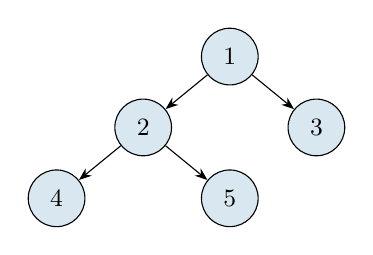
\begin{tikzpicture}[
			level 1/.style={sibling distance=2.2cm},
			level distance=0.9cm,
			edge from parent/.style={draw, -{Stealth[length=1.6mm]}},
			every node/.style={}]
			\node[treenode] (r) {1}
				child {node[treenode] {2} child {node[treenode] {4}} child {node[treenode] {5}}}
				child {node[treenode] {3}};
		\end{tikzpicture}
		\hspace{0.4cm}
		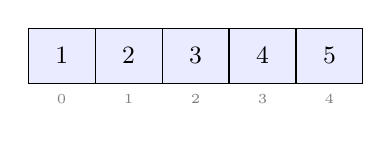
\begin{tikzpicture}[baseline, cell/.style={draw, minimum width=0.85cm, minimum height=0.7cm, fill=blue!8, font=\small}]
			\foreach \val/\idx in {1/0, 2/1, 3/2, 4/3, 5/4} {
				\node[cell] at (\idx*0.85,0) {\val};
				\node[font=\tiny, text=gray] at (\idx*0.85,-0.55) {\idx};
			}
		\end{tikzpicture}
		\vspace{0.1cm}
		\centering\footnotesize e.g. node \texttt{2} at index \texttt{1}: children at \texttt{3}$(=2\cdot1+1)$ and \texttt{4}$(=2\cdot1+2)$ hold \texttt{4} and \texttt{5}.
	\end{frame}

	\begin{frame}[fragile]{Insertion \& Deletion in the Array Representation}
		\begin{columns}[T]
			\begin{column}{0.56\textwidth}
				\begin{lstlisting}
#define MAX 100
int tree[MAX];
int count = 0;      /* number of nodes so far */

/* insert next node in level order */
void insert(int x) {
    if (count == MAX) { printf("Full\n"); return; }
    tree[count++] = x;
}

/* children of node at index i */
int leftChild(int i)  { return 2*i + 1; }
int rightChild(int i) { return 2*i + 2; }
				\end{lstlisting}
			\end{column}
			\begin{column}{0.44\textwidth}
				\begin{itemize}\small
					\item \textbf{Insertion} adds the new value at the next free index (level-order fill).
					\item \textbf{Deletion} of the last node is just \texttt{count-{}-}; deleting an internal node
					usually moves the last node into the gap.
					\item The index formulas let us move between parent and children with \emph{no pointers}.
				\end{itemize}
			\end{column}
		\end{columns}
	\end{frame}

	\begin{frame}{Summary \& What Comes Next}
		\begin{columns}[T]
			\begin{column}{0.5\textwidth}
				\begin{block}{You now know}
					\begin{itemize}\small
						\item Declaring, initializing, and accessing \textbf{structures}.
						\item Using structures with functions (value vs pointer).
						\item \textbf{Self-referential} structures and \textbf{unions}.
						\item What data structures are and their operations.
						\item \textbf{Stacks} (LIFO) and \textbf{queues} (FIFO) via arrays.
						\item \textbf{Trees} and their array representation.
					\end{itemize}
				\end{block}
			\end{column}
			\begin{column}{0.5\textwidth}
				\begin{block}{Practice}
					\begin{itemize}\small
						\item Build a stack-based bracket checker.
						\item Implement a circular queue.
						\item Traverse the array-tree (in-order).
					\end{itemize}
				\end{block}
				\begin{block}{Coming up}
					\small Linked lists, binary search trees, and algorithm analysis.
				\end{block}
			\end{column}
		\end{columns}
	\end{frame}

	%------------------------------------------------
	\begin{frame}
		\centering
		\Huge Thank You
		\vspace{0.5cm}

		\normalsize Questions?
	\end{frame}

	%------------------------------------------------
\end{document}
